\documentclass[12pt]{article}
\usepackage{pslatex} % Font Times New Roman

\usepackage{amsmath,amssymb,amsfonts,fancyhdr,lastpage}
\usepackage{makeidx, graphicx}

\setlength{\textheight}{9.0in}
\setlength{\topmargin}{-.5in}
\setlength{\textwidth}{6.5in}
\setlength{\oddsidemargin}{-.0in}
\setlength{\parskip}{6pt}


\renewcommand{\headrulewidth}{0pt}
\setlength{\headsep}{.35in}
\addtolength{\headheight}{2.5pt} 

\usepackage{graphicx}
\usepackage{fixltx2e}
\usepackage{tikz}

\begin{document}

\title{Methodology for Realizing Graphs in Stable Polycyclic Unsaturated Hydrocarbons}
\author{Aaron Germuth and Alex Aravind \\\\  
Department of Computer Science \\
University of Northern British Columbia \\
E-mail: (germuth,csalex)@unbc.ca}
\maketitle


\begin{abstract}

This report outlines the methodology used to find realistic graphs for classified Kekul\'{e} cells.

\end{abstract}

\section{Introduction}

Certain conjugated hydrocarbons exhibit an electrical switching behavior which could be useful in molecular circuitry. This behavior is completely decided by the Kekul\'e Cell of the molecule's graph. In such graphs, atoms are abstracted as nodes, and chemical covalent bonds as edges. Ports are special nodes which do not need to participate in conjugation, and can connect to the outside world. 

All possible Kekul\'e cells of rank
\footnote{Rank is defined as the amount of ports within a single graph or cell} \textless 7 can be simplified to a cell from Hesselink's \cite{H13} classification.
He also went on to discover graphs for (nearly) every cell in his classification. However, most graphs do not correspond to realistic molecules. We wish to improve upon the classification by providing more accurate graphs.

In order for a graph to be considered 'realistic' we have composed several restrictions:
\begin{enumerate}
\item Interval vertices are restricted to a degree of \textless 4
\item Ports are restricted to a degree of \textless 3
\item Cycles within the graph must be of size \textgreater 4
\item All Graphs must be connected
\item No intersection of edges
\end{enumerate}

With these restrictions we have found a graph for every classification of rank 4 and 5 using methods outlined below: exhaustive search, template molecules, and the editing of existing graphs. 

\section{Exhaustive Search}

Hesselink (Section 4.2) \cite{H13} started with the observation that Kekul\'e cells are monotonic (preserve order) in the set of edges and therefore: 

$E_0 \subseteq E \implies K(V, E_0) \subseteq K(V, E)$

Where V = set of vertices, E = set of edges, and K(V, E) = Kekul\'e cell of graph G = (V,E). 

Every port assignment found in K(V, E\textsubscript{0}) is also found in K(V, E). This implies the possibility that we can start with a smaller graph G\textsubscript{0}, and slowly add edges to approximate K(V, E). If at any point
$E\textsubscript0 \nsubseteq E$, we have failed to find a graph and
the process is repeated with more possible vertices. In order to get a terminating procedure, we fix a finite set V of vertices and a set of edges L, which can be added to the graph. 

This method relies on starting with a smaller subset graph to search from. This graph is obtained by including only the ports as vertices and allowing 'border channels' between the ports. These are edges which have been proven to not effect the Kekul\'e Cell, and therefore can be included. From this small graph edges are slowly added. 

Since we consider all sets E where: 
$$E_0 \subseteq E \subseteq E_0 \cup L$$
the time complexity is already quite large. All possible internal vertex arrangements are added by considering each graph of the isomorphic class of matched graphs. When 8 vertices are used, this class is 10413 graphs long. Considering there are $2^{6*8}$ relations between a set of six vertices and a set of 8, and over 10000 graphs to try, it is unfeasible to attempt to search for any graphs with 8 or more internal vertices.\footnote{Only even sets of vertices are considered due to Lemma 2 of Hesselink Section 3.2 \cite{H13}}

Instead of simply terminating after finding the first applicable graph, we can continue searching until the vertex limit is reached and retrieve all graphs which satisfy the cell. We then prune out graphs with unrealistic degrees on their vertices. This may still result graphs which are unrealistic (such as disjoint), but in most cases we can alleviate this by editing the graph (see Section 4).

\section{Using Known Aromatic Hydrocarbons as Templates}

The greatest disadvantage of last method is its limitation in the amount of vertices. Many polycyclic polyunsaturated hydrocarbons contain upwards of 10 atoms (pyrene, pyracylene, see Figure 1). Not only are molecules such as these stable, but they may be necessary. Adding more nodes to a graph while preserving the cell tends to lower the degree of the nodes, and so larger graphs may be needed to fit all of our restrictions. 

\begin{figure}[ht!]
\centering
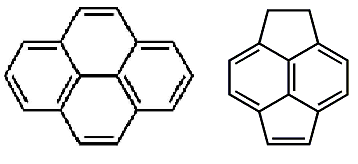
\includegraphics[width=90mm]{largeMolecules.png}
\caption{Two large polycylic aromatic hydrocarbons. From left to right, pyrene, and pyracylene.}
\end{figure}

In this approach we take commonly known conjugated hydrocarbons, and use them as a template. We consider all possible port locations and classify the molecule for each combination. For example, Hesselink \cite{H13} looked at all 14 possible combinations of 5 ports on pyracylene and classified 8 different cells \cite{H13}. 

In order to do this efficiently, we must consider symmetry. Consider the example given above, pyracylene with 5 ports. Since there are 8 nodes in pyracylene which can support a port due to the laws of carbon chemistry (degree of \textless 3), there are 8 positions to put 5 ports. This gives $\binom{8}{5}$ or 46 possible combinations of port locations. However, this can be reduced to only 14 if we consider the symmetry groups of the nodes and trim out combinations which are symmetric.

The advantage to this approach is that one molecule may result in multiple classifications, and we know the molecule is stable. However, we could never look at every one, and it is some what of a matter of luck in picking the right molecule.  

\section{Editing structures}

There has been some literature on methods to change a graph without changing its cell. Hesselink et al \cite{HH13} show a way to split a node of high degree into multiple nodes of lower degree. M.H Van der Veen \cite{v06} classifies a list of operations which can be used to edit structures. Of course, in order to edit a structure you have to have a graph to edit, so this method is normally used in addition to one of the above methods. 

\subsection{Joining Disconnected Graphs}

Some graphs obtained from section 2 are disjoint, as connectedness is not a requirement in the recursive step. Molecules however, must be connected. If an atom is not directly bonded within the molecule, it is not part of that molecule. Luckily, we can use usually connect two disjoint graphs without affecting the cell. If we add internal vertices which must always conjugate 'within' themselves, they will not interfere with the cell. For example, see Figure 1. 

\begin{figure}[ht!]
\centering
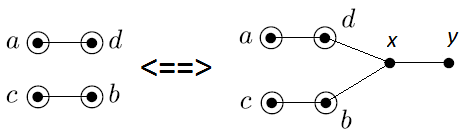
\includegraphics[width=90mm]{disjoint.png}
\caption{Transforming a disjoint graph into a connected one. Ports are represented by encircled nodes.}
\end{figure}

In the right-hand graph of Figure 2, \textit{y} is not a port and so must always contain a double bond. The only other node which is available to form a double bond with \textit{y} is \textit{x}, so in every resonance structure of this molecule x and y will contain a double bond with each other. Therefore \textit{d} or \textit{b} can never form a double bond with their new edge, and the Kekul\'{e} cell has not been changed. This now resembles a stable connected molecule. 

This procedure is similar to \textit{Operation iii} and \textit{Operation vi} of \cite{v06}. 

\subsection{Reducing the degree on all ports}

Sometimes the best graph you can find still has a high degree at one or more nodes. One common strategy is to 'extend' all the ports away by one bond, and leave a new internal vertex at their old position. It is unclear whether this always holds true in all cases, but regardless is a common strategy to reduce the degree. 

Hesselink et al. \cite{HH13} show a technique to converge 3 nodes into one. If the process is done backwards, it can split a node of high degree into two nodes of lesser degree. It can even be done twice, by first merging and then re-splitting, in order to shuffle edges across nodes, similar to \textit{Operation vii} of \cite{v06}. 

\subsection{Removing Steric Hinderance}

Another factor which causes results to not correspond to stable molecules is
steric hinderance between carbons atoms. Carbon is tetrahedral and prefers to bond to 4 identities at approximately 109.5$^\circ$. However, in triangular arrangements such as cyclopropene, the carbon bonds are forced to be 60$^\circ$. In cyclobutadiene, the bonds are 90$^\circ$. However, we can easily avoid such hinderance by again adding  two internal vertices which are conjugated to everything (similiar to \textit{Operation vi} of \cite{v06}). In the case of cyclopropene, we add two vertices to create cyclopentene. With cyclobutadiene, we get benzene (see Figure 3). This is why we restrict cycles within the graph to be of size \textgreater 4. Within a molecule such as cyclopentene, the angles are 108$^\circ$, explaining it's stability. 

\begin{figure}[ht!]
\centering
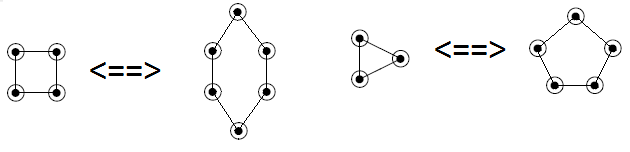
\includegraphics[width=90mm]{cycles.png}
\caption{ Removing steric hinderance by adding additional internal vertices. From left to right, cyclobutadiene, benzene, cyclopropane, cyclopentane}
\end{figure}

\subsection{Adding or Removing Edges}

Based on the nature of Hesselink's classifications, as the Kekule classification 'number' increases (ex. K3 as opposed to K7) the complexity of the cell increases. The number of resonance states and therefore port assignments increases until the last classification which contains every assignment of even length. We can use this fact to help us search for missing graphs. For example, assume you had a graph for K21 and were searching for K23. Since K23 has more port assignments than K21, we can try adding edges to our graph of K21 in order to find K23. This approach is by no means a guarantee, but has been useful in the past.

\section{Current Results}

Insert 7 graphs for rank 4 and 24 graphs for rank 5 here: 
%
%\begin{tikzpicture}
%  [scale=.4,auto=left,every node/.style={circle,fill=blue!15}]
%  \node (n6) at (1,10) {6};
% \node (n4) at (8,5)  {d};
%  \node (n5) at (8,9)  {5};
%  \node (n1) at (2,2)  {a};
%  \node (n2) at (9,6)  {2};
%  \node (n3) at (8,2)  {c};

%  \foreach \from/\to in {n3/n4}
%   \draw (\from) -- (\to);

%\end{tikzpicture}
%

\section{Putting it Together}

All the above logic has been combined into one application which can find stable graphs for nearly every classification of rank 5. The procedure is as follows. First, Hesselink's approach is performed. Instead of simply returning the first graph which satisfies the cell, we keep searching until we have tried all possibilities within the vertex limit. We then parse through our list of applicable graphs. First all graphs are checked for their highest degree. Graphs with a degree more than 3 on normal vertices or more than 2 on ports are removed. 

Next, graphs which are disjoint are fixed. This procedure is outlined in section 4.2. The graph is parsed for detection of 3 cycles (cycles of length 3). The steric hinderance of a 3 cycle is too unstable to be present within a real molecule. For this reason, we extend such cycles to 5 cycles, which are commonly seen in aromatic hydrocarbons. 

We then add to the long list of trimmed graphs based on all the template molecules. If one section has not found an applicable graph at this point, we attempt to add edges. We take every graph from every classification below the missing one, and try to add possible edges to the graph. Only edges which will exceed the maximum degree of the graph are considered. In the case of adding an edge between the ports, the ports can often be 'extended' first to prevent the degree from exceeding our limit. From this, we display the graph with the lowest amount of nodes to the user. (currently in text form).

We want to put all these methods together into one application which can get you realistic graphs for every classification. I believe first it should run Hesselink's program and try to get graphs. If more than one graph is available, the first one found should be viewable, but ideally, all should be viewable somehow. Then, if some haven't been found, we try 10 or so built in molecules. Option should be there to add in your own custom molecule and see if it fits any classification. Finally, if some still aren't found, it should take classifications it already has and try adding/removing edges to get intermediate ones. Some editing will be done i imagine.

\subsection{Current Questions}

Can you get the rank of a cell from it's port assignments. Does every single possible cell with 5 ports have at least one port assignment with e? if not, you must tell the rank of your cell.


\begin{thebibliography}{abrv}

\bibitem{H13} W. H. Hesselink, Graph Theory for alternating hydrocarbons with attached ports. Indagationes Mathematicae, Elsevier, 24:115141, 2013.
\bibitem{HH13} W.H. Hesselink, J.C. Hummelen, H.T. Jonkman, H.G. Reker, G.R. Renardel de Lavalette, M.H. van der Veen, Kekule Cells for Molecular Computation. Cornell University Library Online, 2013.
\bibitem{v06} M.H. van der Veen. $\pi$-Logic. PhD thesis, University of Groningen, May 2006.
\bibitem{HK88} A.J. Heeger, S. Kivelson, J.R. Schrieffer, and W.-P Su. Solitons in conducting polymers, Rev. Mod. Phys.,60:781, 1988.

\end{thebibliography}

\end{document}
